\documentclass[oneside, 11pt]{article}

\usepackage[T1]{fontenc}
\usepackage[utf8]{inputenc}
\usepackage[english]{babel}
\usepackage{enumerate}
\usepackage{isotope}


\usepackage{fouriernc}
\usepackage[detect-all, binary-units, separate-uncertainty=true,
            per-mode=symbol, retain-explicit-plus, retain-unity-mantissa=false]{siunitx}

\usepackage{setspace}
\setstretch{1.2}

\setlength{\parskip}{\smallskipamount}
\setlength{\parindent}{0pt}

\usepackage[headheight=14pt]{geometry}
\geometry{marginparwidth=0.5cm, verbose, a4paper, tmargin=3cm, bmargin=3cm,
          lmargin=2cm, rmargin=2cm}

\usepackage{float}

\usepackage[fleqn]{amsmath}
\numberwithin{equation}{section}
\numberwithin{figure}{section}

\usepackage{graphicx}
\graphicspath{{images/}{../../../images/}}

\usepackage{tikz}
\usetikzlibrary{shapes}
\usetikzlibrary{plotmarks}

\newcounter{Exercise}
\setcounter{Exercise}{1}
\usepackage{xcolor}
\definecolor{shadecolor}{gray}{0.9}
\usepackage{framed}
\usepackage{caption}

\usepackage{url}


\usepackage{fancyhdr}
\pagestyle{fancy}
\fancyhf{}
\rhead{\thepage}
\renewcommand{\footrulewidth}{0pt}
\renewcommand{\headrulewidth}{0pt}

\fancypagestyle{firststyle}
{
    \fancyhf{}
    \rhead{\thepage}
    \cfoot{\includegraphics[height=30pt]{HiSPARClogo}}
    \rfoot{\includegraphics[height=25pt]{CCbysa}}
    \lfoot{
\includegraphics[height=30pt]{NIKHEFlogo}}
    \renewcommand{\footskip}{50pt}
    \renewcommand{\footrulewidth}{0.1pt}
    \renewcommand{\headrulewidth}{0pt}
}

\newcommand{\figref}[1]{Figuur~\ref{#1}}

\newcommand{\hisparc}{\textsmaller{HiSPARC}\xspace}
\newcommand{\kascade}{\textsmaller{KASCADE}\xspace}
\newcommand{\sapphire}{\textsmaller{SAPPHiRE}\xspace}
\newcommand{\jsparc}{\textsmaller{jSparc}\xspace}
\newcommand{\hdf}{\textsmaller{HDF5}\xspace}
\newcommand{\aires}{\textsmaller{AIRES}\xspace}
\newcommand{\csv}{\textsmaller{CSV}\xspace}
\newcommand{\python}{\textsmaller{PYTHON}\xspace}
\newcommand{\corsika}{\textsmaller{CORSIKA}\xspace}
\newcommand{\labview}{\textsmaller{LabVIEW}\xspace}
\newcommand{\daq}{\textsmaller{DAQ}\xspace}
\newcommand{\adc}{\textsmaller{ADC}\xspace}
\newcommand{\hi}{\textsc{h i}\xspace}
\newcommand{\hii}{\textsc{h ii}\xspace}
\newcommand{\mip}{\textsmaller{MIP}\xspace}
\newcommand{\hisparcii}{\textsmaller{HiSPARC II}\xspace}
\newcommand{\hisparciii}{\textsmaller{HiSPARC III}\xspace}

\DeclareSIUnit{\electronvolt}{\ensuremath{\mathrm{e\!\!\:V}}}

\DeclareSIUnit{\unitsigma}{\ensuremath{\sigma}}
\DeclareSIUnit{\mip}{\textsmaller{MIP}}
\DeclareSIUnit{\adc}{\textsmaller{ADC}}

\DeclareSIUnit{\gauss}{G}
\DeclareSIUnit{\parsec}{pc}
\DeclareSIUnit{\year}{yr}




%document details
\author{N.G. Schultheiss \\ translated and adapted by K. Schadenberg}
\date{}
\title{Data Processing - Non-periodic Data}


\begin{document}
\maketitle

\section{Introduction}
This module is a continuation of `Periodic data' in which the downloading and importing of data was explained. The previous module also showed how to analyse data when there is some periodic dependence. But you might also want to look at the influence of phenomena which do not have a clearly repeating pattern; the influence of weather, e.g. temperature, ambient pressure, and cloud cover, or other non-repeating effects. The temperature might roughly follow the pattern of day and night, but lightning clearly does not.

\section{Change of Occurrence}
Before we can determine if cosmic radiation or air showers are influenced by a certain phenomena we first need to make sure the phenomenon actually occurred. In some cases we know with 100\% certainty that something happened, but in other cases we are not so sure, then we might only know the odds of it happening; the probability $P()$.

Lets start by looking at an easy example. We have been observing the weather for an entire day and recorded the times at which there were  thunderstorms. The results are shown in figure~\ref{fig:thunder}.

\begin{figure}\begin{center}
\begin{picture}(0,0)%
\includegraphics{thunder}%
\end{picture}%
\setlength{\unitlength}{4144sp}%
%
\begingroup\makeatletter\ifx\SetFigFont\undefined%
\gdef\SetFigFont#1#2#3#4#5{%
  \reset@font\fontsize{#1}{#2pt}%
  \fontfamily{#3}\fontseries{#4}\fontshape{#5}%
  \selectfont}%
\fi\endgroup%
\begin{picture}(7037,2245)(-194,-1394)
\end{picture}%
\caption{The odds of thunderstorms.}\label{fig:thunder}
\end{center}\end{figure}

This figure is only part of the story, we also need to look at the odds of `no thunderstorms'. The probability of no thunderstorms occurring are shown in figure~\ref{fig:no_thunder}. %Because there are only two options in this example, either there is thunder or not, figure~\ref{fig:no_thunder} is the exact opposite of figure~\ref{fig:thunder}

\begin{figure}\begin{center}
\begin{picture}(0,0)%
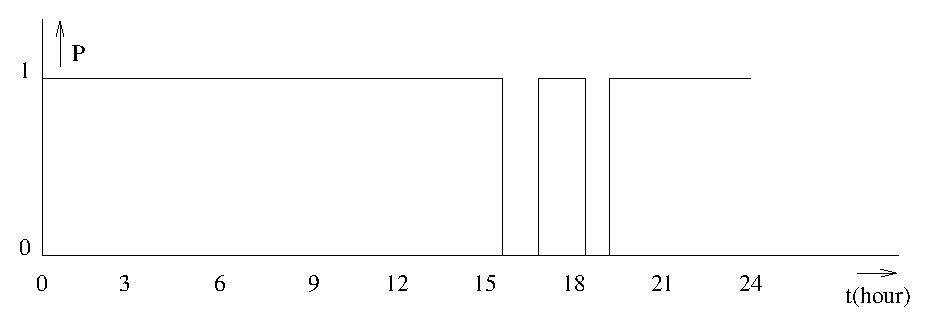
\includegraphics{no_thunder}%
\end{picture}%
\setlength{\unitlength}{4144sp}%
%
\begingroup\makeatletter\ifx\SetFigFont\undefined%
\gdef\SetFigFont#1#2#3#4#5{%
  \reset@font\fontsize{#1}{#2pt}%
  \fontfamily{#3}\fontseries{#4}\fontshape{#5}%
  \selectfont}%
\fi\endgroup%
\begin{picture}(6945,2245)(-194,-1394)
\end{picture}%
\caption{The odds of no thunderstorms.}\label{fig:no_thunder}
\end{center}\end{figure}

\begin{shaded}
\textbf{Exercise \theExercise \stepcounter{Exercise}} : Explain why the following equality is true:
\begin{equation}
P(\mbox{Thunderstorms})+P(\mbox{No thunderstorms}) = 1
\end{equation}
\end{shaded}

Lets assume cosmic radiation is not influenced by the weather. We therefore create fictitious measurement data, as shown in figure~\ref{fig:constant}, of the day we observed the thunderstorms  with no variation during the day.\footnote{We have also `corrected' our fictitious data for any known and unknown variations other than thunderstorms.} 

\begin{figure}\begin{center}
\begin{picture}(0,0)%
\includegraphics{constant}%
\end{picture}%
\setlength{\unitlength}{4144sp}%
%
\begingroup\makeatletter\ifx\SetFigFont\undefined%
\gdef\SetFigFont#1#2#3#4#5{%
  \reset@font\fontsize{#1}{#2pt}%
  \fontfamily{#3}\fontseries{#4}\fontshape{#5}%
  \selectfont}%
\fi\endgroup%
\begin{picture}(7260,2245)(-509,-1394)
\end{picture}%
\caption{A constant flux of cosmic radiation.}\label{fig:constant}
\end{center}\end{figure}

When investigating the influence of thunderstorms we would compare the measurements during thunder with the data taken from when there were no thunderstorms. To do this you multiply figure~\ref{fig:constant} with figure~\ref{fig:thunder} and add all the values to obtain the number of coincidences for when there were thunderstorms and with figure~\ref{fig:no_thunder} to obtain the data without thunderstorms. It now seems as though there is a much higher change to observe cosmic radiation in nice weather. There is one final step needed to correct this.

\begin{shaded}
\textbf{Exercise \theExercise \stepcounter{Exercise}} : Figure~\ref{fig:thunder} and \ref{fig:no_thunder} show that is far more likely to have nice weather than to have thunderstorms. How does one need to use this information to determine whether or not thunderstorms influence cosmic radiation.

\emph{Hint: What does the area underneath the lines in figure~\ref{fig:thunder} and \ref{fig:no_thunder} tell you?}
\end{shaded}

\section{Using a Spreadsheet}
Processing non-periodic data can be done using a spreadsheet. The following steps are written for our thunderstorm example, but can be easily modified and expanded to tackle other problems.

\begin{enumerate}[1]
\item Download the relevant (coincidence) data from the HiSPARC website and import it into the spreadsheet.
\item Calculate the probability of thunderstorms for every hour and place the results in a separate column `Thunder'. If there was a thunderstorm lasting 15 minutes during an hour, the probability $P(\mbox{Thunderstorm}) = 0.25$.
\item Calculate the probability of no thunderstorms using\\ $P(\mbox{Thunderstorms})~+~P(\mbox{No thunderstorms}) = 1$ and place it in a separate column labelled `No thunder'.
\item Calculate the sum of the columns 'Thunder' and 'No thunder'.
\item For every time interval (hour) calculate $\mbox{\#coincidences} ~\cdot~  P(\mbox{Thunderstorms})$ and \\$\mbox{\#coincidences} ~\cdot~ P(\mbox{No thunderstorms})$, place the results in two new separate columns.
\item Calculate the sum of $\mbox{\#coincidences} ~\cdot~ P(\mbox{Thunderstorms})$ and divide this by the sum of the column 'Thunder', this is 'Chance of Thunder'.
\item In a similar fashion calculate the 'Chance of No thunder' by calculating the sum of $\mbox{\#coincidences} ~\cdot~ P(\mbox{No thunderstorms})$ and divide this by the sum of the column 'No thunder'.
\item Compare the values for 'Chance of Thunder' and 'Chance of No thunder', the largest wins.
\end{enumerate}

\begin{shaded}
\textbf{Exercise \theExercise \stepcounter{Exercise}} : Some HiSPARC stations are equipped with a weather station. Temperature and ambient pressure data are sent along the with other data to the NIKHEF in Amsterdam and the results can be downloaded from the same data page. Station 501 is such a station, an example of its data page is shown in figure~\ref{fig:501_weather}.

What problems arise when we try to investigate the dependence of cosmic radiation on ambient pressure when we use the data from station 501?
\end{shaded}

\begin{figure}\begin{center}
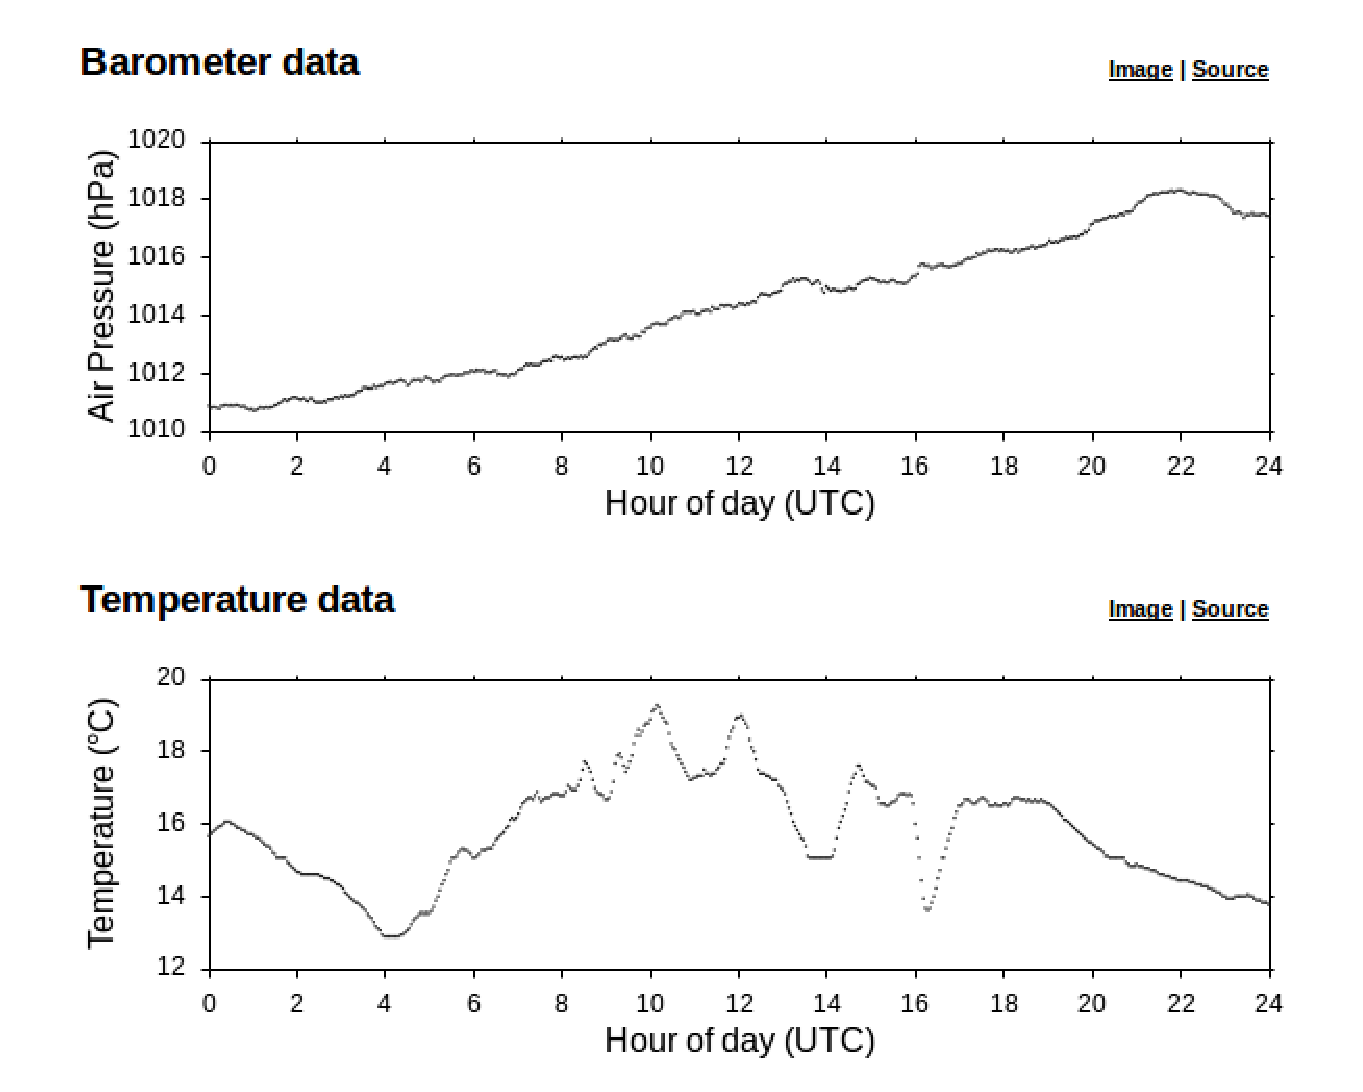
\includegraphics[scale=0.7]{501_weather.eps}
\caption{Weather data from station 501 on the 1st of July 2012.}\label{fig:501_weather}
\end{center}\end{figure}

Figure~\ref{fig:501_weather} shows the weather data from station 501, like the other graphs on the data page these graph have a link to the source to download the data. The results are written in a .csv file but in a slightly different way than the detector data. The temperature and ambient pressure are measured every second. These seconds are not counted for every day, but since the 1st of January 1970. This is known as POSIX time.\footnote{Explaining all the details about POSIX or Unix time and why it does not include leap seconds for instance goes beyond the scope of this text. On the internet multiple methods can be found to convert POSIX time into something we can all understand.} Our coincidence is per hour, so we need to convert the weather data to match this.\footnote{This is called 'rebinning', all the data was placed into bins (sort of like buckets) 1 second wide, now we want to place them into bins 3600 seconds wide.}

\section{Correlation between Two Graphs}
Looking for correlations between two graphs can be done using the steps described in the previous section. But there is a faster and smarter way of doing this. In the following example we will look at the possible connection between cosmic radiation and ambient pressure.

\begin{enumerate}[1]
\item Download the coincidence data and import it into a spreadsheet.
\item Download the weather data for the same time interval and also import it into a spreadsheet. If needed convert the data so it can be used with the coincidence data (rebinning).
\item Determine the average pressure for the entire time interval.
\item Calculate the difference between the instantaneous pressure and the average pressure for each measurement point, place these values in a separate column.
\item Multiply the deviation from the average with the number of coincidences for each time interval. Place the result in a separate column.
\item Calculate the sum of this final column. Is the result a positive number, then an increase in pressure is associated with an increase in cosmic radiation. Is the result negative, then the reverse is true. 
\end{enumerate}

\begin{shaded}
\textbf{Exercise \theExercise \stepcounter{Exercise}} : Compare the procedure above with the procedure from the previous section. Do they give the same result?\end{shaded}

\end{document}
